\documentclass[aspectratio=169]{beamer}
\usepackage[T1]{fontenc} 
\usepackage[default]{sourcesanspro}
\usepackage{fourier}
\usepackage{hyperref}
\usepackage{latexsym,amsmath,xcolor,multicol,booktabs,calligra}
\usepackage{graphicx,pstricks,listings,stackengine}
\usepackage{lipsum}
\usepackage{wrapfig}
\usepackage{url}
\usepackage{subcaption}

\usepackage{etoolbox}

\input{math_commands.tex}

\author{\underline{Yan Lin}, Jonas A. Finkler, Tao Du, Morten M. Smedskjaer, Jilin Hu}
\title{AMDEN: Amorphous Materials DEnoising Network}
\subtitle{Generation of Amorphous Materials with Tailored Properties}
\institute{
  \href{mailto:lyan@cs.aau.dk}{lyan@cs.aau.dk}\\
  \href{https://www.en.tech.aau.dk/research/research-groups/data-engineering-science-og-systems-dess}{Department of Computer Science} \\
  \href{https://www.en.aau.dk/}{Aalborg University} \\
}
\date{\small Augest 10, 2025}
\usepackage{AAU}

% Remove navigation buttons
\setbeamertemplate{navigation symbols}{}

% defs
\def\cmd#1{\texttt{\color{red}\footnotesize $\backslash$#1}}
\def\env#1{\texttt{\color{blue}\footnotesize #1}}
% set colors
\definecolor{aauyellow}{RGB}{167, 131, 55}
\definecolor{aaublue}{RGB}{32, 26, 78}
\definecolor{aaured}{RGB}{152, 43, 28}

\def\emphasis#1{\color{aaured}#1}


\lstset{
  basicstyle=\ttfamily\small,
  keywordstyle=\bfseries\color{deepblue},
  emphstyle=\ttfamily\color{deepred},    % Custom highlighting style
  stringstyle=\color{deepgreen},
  numbers=left,
  numberstyle=\small\color{halfgray},
  rulesepcolor=\color{red!20!green!20!blue!20},
  frame=shadowbox,
}

%- --- --- --- --- --- --- --- --- --- --- --- --- --- --- --- 
\begin{document}

\begin{frame}[plain,noframenumbering]
  \titlepage
  \vspace*{-0.6cm}
  \begin{figure}[htpb]
    \begin{center}
      \begin{minipage}{0.4\textwidth}
        \raggedleft
        \includegraphics[keepaspectratio, height=.8cm]{aau-logo-left-uk.pdf}
      \end{minipage}
      \hspace{.4cm}
      \begin{minipage}{0.4\textwidth}
        \raggedright
        \includegraphics[keepaspectratio, height=.8cm]{figures/vf.png}
      \end{minipage}
    \end{center}
  \end{figure}
\end{frame}

% \begin{frame}    
% \tableofcontents[sectionstyle=show,
% subsectionstyle=show/shaded/hide,
% subsubsectionstyle=show/shaded/hide]
% \end{frame}

\section{Background}

\begin{frame}{Discovering Amorphous Materials with Desired Properties}
  \begin{block}{Trial-and-error}
    Screen through the design space until samples with desired properties are found.

    \begin{figure}[htpb]
      \vspace{-0.3cm}
      \begin{center}
        \includegraphics[keepaspectratio, height=0.25\textheight]{figures/screen.pdf}
      \end{center}
      \vspace{-0.3cm}
    \end{figure}
  \end{block}

  \begin{itemize}
    \item Techniques like high-throughput screening, computer simulation, machine learning-based property prediction can be used to speed up the process
    \item Inevitably, a large number of material samples need to be created/generated, leading to \textbf{high manpower, material, and time costs}
  \end{itemize}
\end{frame}

\begin{frame}{Discovering Amorphous Materials with Desired Properties}
  \begin{block}{Inverse Design}
    Begin with desired properties and determine the atomic configurations to achieve them.
    \begin{figure}[htpb]
      \vspace{-0.3cm}
      \begin{center}
        \includegraphics[keepaspectratio, height=0.25\textheight]{figures/generation.pdf}
      \end{center}
      \vspace{-0.3cm}
    \end{figure}

    \begin{itemize}
      \item Far fewer material samples need to be screened, saving costs
      \item Has the potential to significantly speed up the discovery of novel amorphous materials
    \end{itemize}
  \end{block}

  \vspace{1em}
  \centering
  \emphasis{How do we achieve inverse design of amorphous materials?}
\end{frame}

\begin{frame}{Generative Modeling with Diffusion Models}
  A family of machine learning frameworks that \textbf{generate data from random noise by denoising the data step-by-step.}
  \begin{figure}[htbp]
    \includegraphics[keepaspectratio, width=0.8\linewidth]{figures/ddpm.png}
    \caption{Image generation process of diffusion models\footnote{\tiny Ho, Jonathan and Jain, Ajay and Abbeel, Pieter. "Denoising Diffusion Probabilistic Models." NeurIPS (2020).}}
  \end{figure}

  \begin{itemize}
    \item Huge success and widely adopted in image and video generation
    \item Inspired lots of efforts in inverse design of crystalline materials and molecules\footnote{\tiny Zeni, Claudio, et al. "A generative model for inorganic materials design." Nature (2025).}, but its adaptation in amorphous materials are understudied
  \end{itemize}
\end{frame}


\section{Methodology}

\begin{frame}{Generative Modeling of Amorphous Materials}
  Start from an initial state of the sample, adjust its atomic positions and elements step-by-step towards the final state.
  \begin{itemize}
    \item Similar to a simulation pipeline but the atoms are not driven by energy and force
    \item Instead, a \textit{neural network} predicts the movements of atoms at each step conditioned on the desired properties
  \end{itemize}
  \begin{figure}
    \centering
    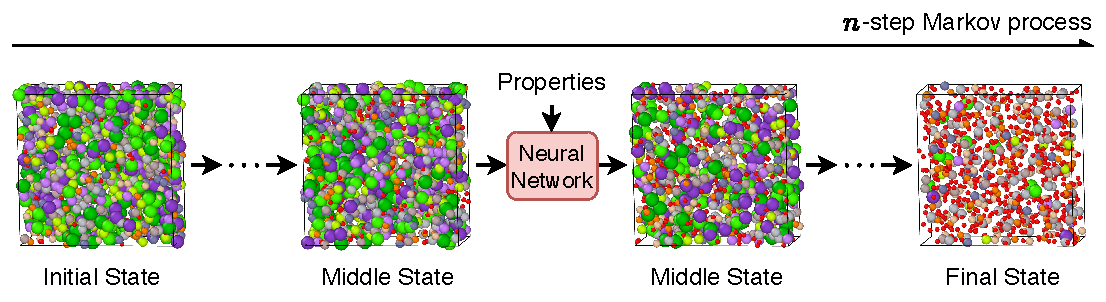
\includegraphics[width=\linewidth]{figures/process.pdf}
  \end{figure}
\end{frame}

\begin{frame}{Neural Network for Generative Modeling}
  \begin{itemize}
    \item Input: Current state of an amorphous material sample at each step, and the desired properties
    \item Output: State of the sample at the next step
  \end{itemize}
  \begin{figure}
    \centering
    \includegraphics[width=.8\linewidth]{figures/network-problem.pdf}
  \end{figure}
\end{frame}

\begin{frame}{Representation of Amorphous Material Samples}
  \begin{columns}
    \begin{column}{0.6\textwidth}
      Representing one amorphous material sample as a tuple $x=(\mC, \mX, \mE)$.

      \begin{itemize}
        \item $\mC \in \mathbb R^{3\times 3}$ are the lattice vectors
        \item $\mX \in \mathbb R^{N\times 3}$ are the atomic positions
        \item $\mE \in \mathbb R^{N\times d}$ are the element one-hot embeddings
      \end{itemize}

      And its properties as a vector $\vy$ where each value is a scalar property.
    \end{column}
    \begin{column}{0.4\textwidth}
      \begin{figure}
        \centering
        \includegraphics[width=\linewidth]{figures/sample-rep.pdf}
      \end{figure}
    \end{column}
  \end{columns}
\end{frame}

\begin{frame}{Equivariant Neural Network Architecture}
  \textbf{Update the positions and elements of atoms} while preserving the geometric equivariance of amorphous material samples.
  \begin{figure}
    \centering
    \includegraphics[width=\linewidth]{figures/network.pdf}
  \end{figure}

  \begin{itemize}
    \item A graph structure of each sample where node and edge features are invariant to permutation and translation
    \item EGNN\footnote{\tiny Satorras, Vıctor Garcia, Emiel Hoogeboom, and Max Welling. "E (n) equivariant graph neural networks." ICLR (2021).} backbone whose update to each sample is invariant
  \end{itemize}
\end{frame}

\begin{frame}{Reversible Generation Process}
  We cannot train a neural network with the generation process alone.

  \begin{figure}
    \centering
    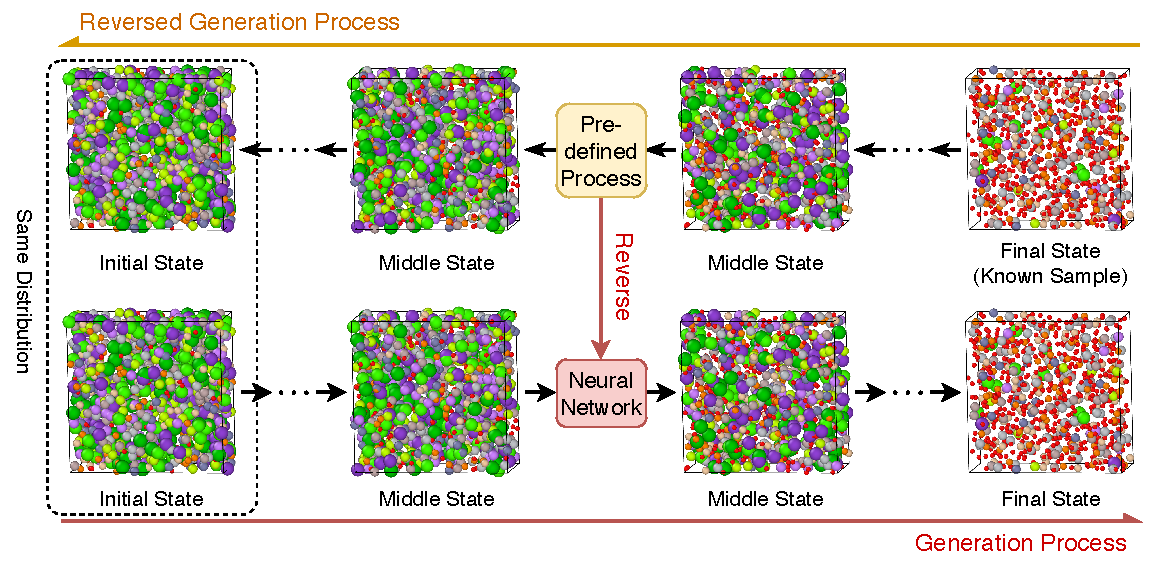
\includegraphics[width=.9\linewidth]{figures/reverse-process.pdf}
    \vspace{-0.3cm}
  \end{figure}

  A reversed generation process providing ground truth for training.
\end{frame}

\begin{frame}{Denoising Generation Process}
  \begin{itemize}
    \item The reversed generation process gradually adds Gaussian noise to the sample until pure noise at the initial state
    \item The neural network learns to remove the noise added in each step
    \item The generation process can start from an initial state of pure Gaussian noise
  \end{itemize}

  \begin{figure}
    \centering
    \includegraphics[width=.8\linewidth]{figures/denoising.pdf}
  \end{figure}
\end{frame}

\begin{frame}{Density Control in the Generation Process}
  \begin{block}{Importance of density control}
    \begin{itemize}
      \item Density in amorphous materials is a key parameter that affects numerous properties
      \item Being able to control the density during generation is essential for generating materials with certain property targets
    \end{itemize}
  \end{block}

  \begin{block}{Limitation of diffusion models}
    \begin{itemize}
      \item Diffusion models manipulate data by adding/removing noise from data — changing the position and element of each atom
      \item \textbf{Adding or removing atoms from the system will be technically challenging for diffusion models}
    \end{itemize}
  \end{block}
\end{frame}

\begin{frame}{Density Control via Ghost Atoms}
  \textbf{Framing the density control problem as changing elements of atoms.}
  % Keep the total number of atoms in a sample static, but enable density control through manipulating the number of ghost atoms.
  \begin{itemize}
    \item Ghost atoms are added to each material sample so that the density (number of atoms per unit volume) of all samples reaches one target maximum value
    \item Ghost atoms are treated as normal atoms by the model but assigned a special element class and removed in the final generated samples
    \item The model can control the density during generation by increasing/decreasing the proportion of atoms with the special element type
  \end{itemize}

  \begin{figure}
    \centering
    \includegraphics[width=\linewidth]{figures/process-ghost.pdf}
  \end{figure}
\end{frame}


\section{Results}

\begin{frame}{Generation of Amorphous Silica}
  With desired \textbf{shear modulus} and \textbf{average ring size} that are dependent on the samples' structures and densities.

  \begin{figure}
    \centering
    \begin{subfigure}{0.45\textwidth}
      \centering
      \includegraphics[width=\linewidth]{figures/SiO2-G.pdf}
      \caption{Accuracy of shear modulus of generated samples}
    \end{subfigure}
    \hfill
    \begin{subfigure}{0.45\textwidth}
      \centering
      \includegraphics[width=\linewidth]{figures/SiO2-RSD.pdf}
      \caption{Accuracy of average ring size of generated samples}
    \end{subfigure}
  \end{figure}
\end{frame}

\begin{frame}{Generation of Multi-element Glass}
  With desired \textbf{Young's modulus} and \textbf{Lithium ratio} that are largely dependent on samples' compositions.

  \begin{figure}
    \centering
    \begin{subfigure}{0.45\textwidth}
      \centering
      \includegraphics[width=\linewidth]{figures/bmp_Li.pdf}
      \caption{Distribution of Lithium ratio of training data and generated samples (with target being 0.15)}
    \end{subfigure}
    \hfill
    \begin{subfigure}{0.45\textwidth}
      \centering
      \includegraphics[width=\linewidth]{figures/bmp_E.pdf}
      \caption{Accuracy of Young's modulus of generated samples}
    \end{subfigure}
  \end{figure}
\end{frame}

\begin{frame}{Generation of Multi-element Glass}
  \begin{columns}[T]
    \begin{column}{0.5\textwidth}
      \begin{itemize}
        \item The flattening at both ends is primarily the result of extrapolation
        \item The Young's modulus of generated samples tend to be smaller than targets
        \item Requenched samples that are simulated with the compositions of generated samples align better with targets
        \item \textbf{The model is able to generate compositionally accurate samples but falls short in generating structures accurately}
      \end{itemize}
    \end{column}
    \begin{column}{0.5\textwidth}
      \begin{figure}
        \includegraphics[width=\linewidth]{figures/bmp_E.pdf}
      \end{figure}
    \end{column}
  \end{columns}
\end{frame}

\begin{frame}{Generation of Amorphous Silicon}
  Trained with a-Si simulated with different thermal histories and perform generation.
  \vspace{-0.5em}
  \begin{figure}
    \centering
    \begin{subfigure}{0.47\textwidth}
      \centering
      \includegraphics[width=\linewidth]{figures/Si-opt-rdf.pdf}
      \vspace{-2.5em}
      \caption{RDF of training (solid) vs. generated (dashed) samples}
    \end{subfigure}
    \hfill
    \begin{subfigure}{0.47\textwidth}
      \centering
      \includegraphics[width=\linewidth]{figures/Si-opt-energy.pdf}
      \vspace{-2.5em}
      \caption{Potential energy distribution of training vs. generated samples}
    \end{subfigure}
  \end{figure}
  \vspace{-1.5em}
  This further demonstrates that \textbf{the model is unable to generate low-energy structures derived from relaxation processes.}
\end{frame}

\begin{frame}{Limitations}
  \begin{block}{Generation of samples with relaxed structures}
    \textbf{Unable to generate amorphous materials with relaxed structures accurately}, an inherent limitation of diffusion models.
  \end{block}

  \begin{block}{Real-world synthesis of generated samples}
    New synthesis techniques are needed to fully take advantage of the generated atomic configurations.
  \end{block}

  \vspace{1em}
  \centering
  \emphasis{\textbf{Further discussion and solutions: stay tuned for the next presentation!}}
\end{frame}


\appendix

\begin{frame}[plain,noframenumbering]
  \begin{center}
    {\large Thank you!}
    \vspace{1cm}
    \\[0.5em]
    {\small \href{mailto:lyan@cs.aau.dk}{lyan@cs.aau.dk} \\
    \href{https://www.yanlincs.com}{www.yanlincs.com}}
  \end{center}
\end{frame}

  \end{document}
